\documentclass[11pt]{article}

\usepackage{graphicx}
\usepackage{multirow}
\usepackage{amssymb}
\usepackage{amsmath}
\usepackage[left = 2cm, right = 2cm, top = 2cm, bottom = 2cm]{geometry}
\usepackage{hyperref}
\usepackage{xcolor}
\usepackage{physics}
\usepackage{soul}
\usepackage{subcaption}
\usepackage{verbatim}
\usepackage{listings}
\usepackage{verbatimbox}


\lstset{basicstyle=\ttfamily,
columns=fullflexible,
frame=single,
breaklines=true,
postbreak=\mbox{\textcolor{red}{$\hookrightarrow$}\space},
language=C++}

\definecolor{red2}{RGB}{255, 49, 49}
\definecolor{green2}{RGB}{144, 238, 144}
\definecolor{purple2}{RGB}{150, 111, 214}
\newcommand{\hlyellow}[1]{{\sethlcolor{yellow}\hl{#1}}}
\newcommand{\hlgreen}[1]{{\sethlcolor{green2}\hl{#1}}}
\newcommand{\hlred}[1]{{\sethlcolor{red2}\hl{#1}}}
\newcommand{\hlpurple}[1]{{\sethlcolor{purple2}\hl{#1}}}

\bibliographystyle{plain}%abbrv} % We choose the "plain" reference style

\title{Notes on Silvaco TCAD Simulations}
% \author{Danush Shekar\\ Supervised by Dr. Zhenyu Ye and Dr. Corrinne Mills}
\date{\today}

\begin{document}

\maketitle
\tableofcontents

\newpage

%\abstract{}%This is my attempt in saving an account of all tips/tricks, notes, and discussions of the simulation tools I have used (mostly related to HEP simulations). In theory, this is also a note to questions and answers I encountered while I studied the subject, and that this notebook should serve as a reference for the doubts my mind stumbles upon in the future.}

\subsection*{Colour legend}
This document will follow a highlighting scheme where text highlighted in different colors mean the following:
\newline
\hlyellow{Yellow coloured text} - Doubts, or sentences that are to be clarified/understood later.\newline
\hlgreen{Green coloured text} - Some takeaways.\newline
%\hlred{Red coloured text} - Mistakes/typos.\newline
\hlpurple{Purple coloured text} - Interesting and unique points, that often are not mentioned explicitly in textbooks/literature.

\section{About}
Silvaco TCAD is one of the major commercial softwares in the current market that offer tools for the simulation of silicon devices. This note in particular will focus on the tools that facilitate the simulation of Silicon sensors utilized in high energy physics experiments. Particular focus will be towards Athena and Atlas. Athena is a "device-technology" simulation tool, and is widely used for simulating the electrical behavior of semiconductor devices. Athena on the other hand, is a "process-technology" simulation tool. It focuses on the simulation of the manufacturing processes involved in creating semiconductor devices, including deposition, etching, diffusion, etc. Both tools are often used hand-in-hand to offer a comprehensive study of the device to be manufactured.

\section{Atlas}
The primary reference used is Silvaco's Atlas User's Manual \cite{silvaco-atlas}. Infact, this section will be a condensed version of the User's Manual, the only differences being the highlighting of parts relevant+useful for Silicon detector simulations, and additional examples provided by the authors. The workflow as given in \cite{silvaco-atlas} is shown below in Figure \ref{fig:atlas-workflow}. In a very primitive sense: we provide inputs to Atlas through Athena output files, and code in DeckBuild. Atlas then provides outputs that can be visualized in TonyPlot. Most of the following subsections will involve working in the DeckBuild level.

\begin{figure}[h]
    \centering
    \frame{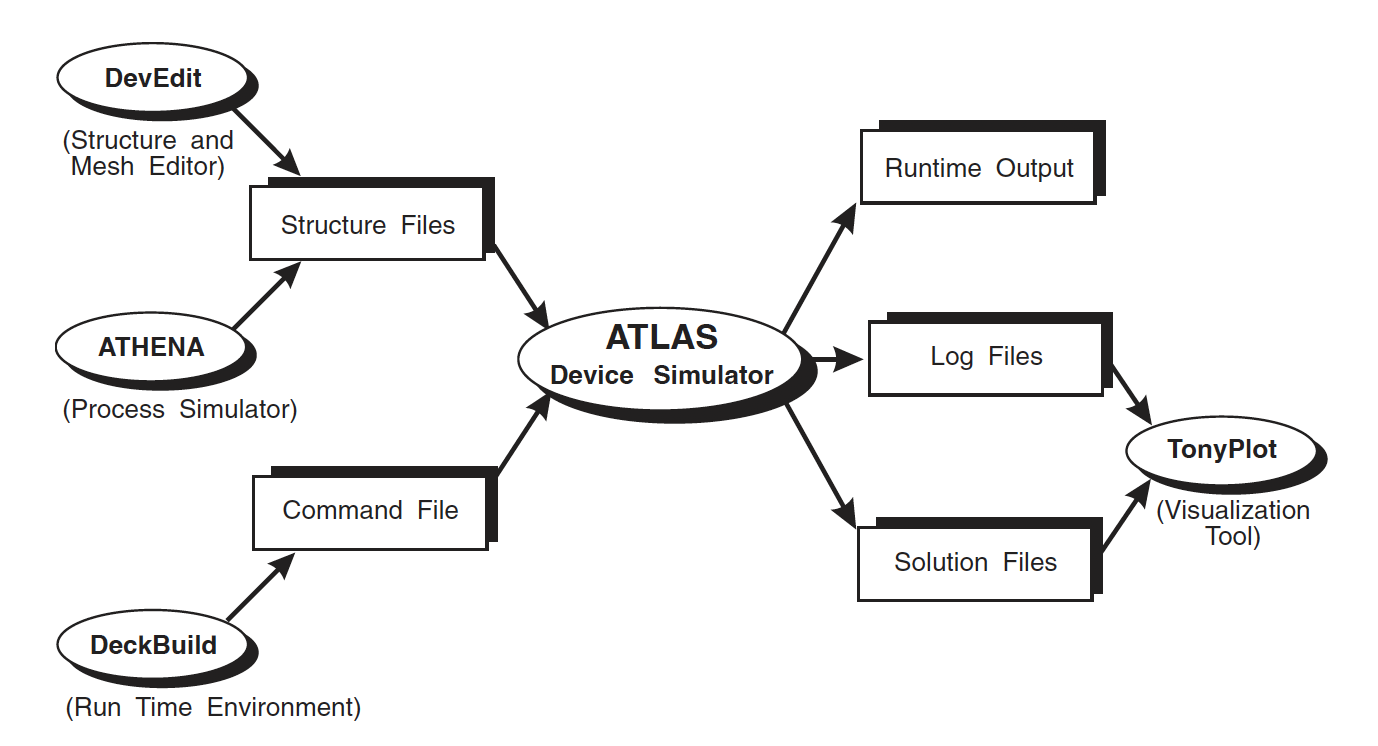
\includegraphics[width=4in]{Images/atlas-input-output.png}}
    \caption{Source: \cite{silvaco-atlas}}
    \label{fig:atlas-workflow}
\end{figure}
Every code line for Atlas will be of the following form: 
\begin{verbatim}
    <STATEMENT> <PARAMETER>=<VALUE>
\end{verbatim}
An example of a statement line is: 
\begin{verbatim}
    DOPING UNIFORM N.TYPE CONCENTRATION=1.0e16 REGION=1
\end{verbatim} 
The statement is DOPING, and all other items are parameters of the DOPING statement. UNIFORM and N.TYPE are logical parameters. Their presence on the line sets their values to true. Otherwise, they take their default values (usually false). CONCENTRATION is a parameter with floating point input. REGION is a parameter taking integers as input.
\newline A crucial thing to note in Atlas code is the order of which statements need to be called in. 
\begin{figure}[h]
    \centering
    \frame{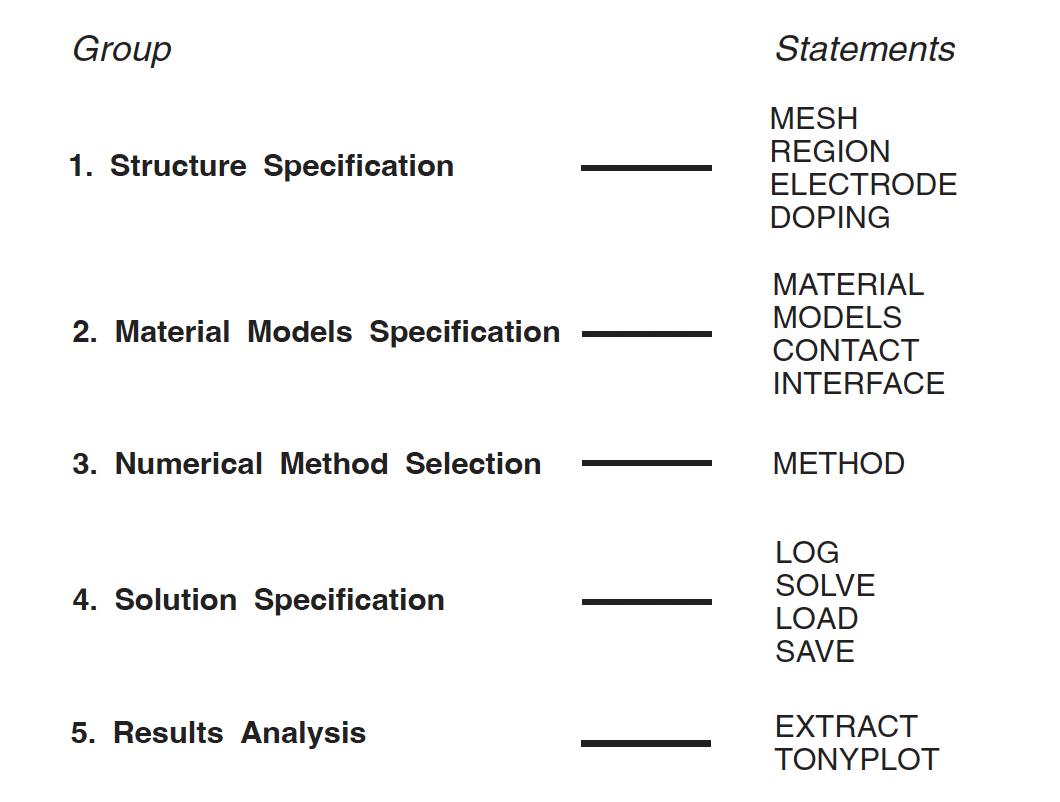
\includegraphics[width=4in]{Images/atlas-statement-order.png}}
    \caption[]{Ordering of statements in Atlas. Source: \cite{silvaco-atlas}}
    \label{fig:atlas-statement-order}
\end{figure}
Typically the spatial units are in microns.
\newline Chapter 21 (Statements) of \cite{silvaco-atlas} contains the syntax and parameter information of most, if not all statements used in Silvaco TCAD simulations.

\subsection{Meshing!}

\subsubsection{Circular mesh}
Some structures can benefit more with a circular mesh than a rectangular mesh, we have been working with, until now. An example of how circular meshes can be defined in Atlas is shown below:
\begin{verbatim}
    MESH CIRCULAR
    R.MESH LOC=0.0 SPAC=0.05
    R.MESH LOC=0.2 SPAC=0.05
    R.MESH LOC=0.35 SPAC=0.025
    R.MESH LOC=0.4 SPAC=0.01
    A.MESH LOC=0 SPAC=30
    A.MESH LOC=360 SPAC=30
\end{verbatim}
The compiler is informed that the mesh will be a circular in the first mesh definition command. The commands that follow are locations and spacings of the mesh the user wants, which is similar to the rectangular meshes (X, Y), except, this time, we are working in circular coordinates (radius$\equiv$R, theta$\equiv$A).

\subsubsection{Regrid/remesh}
After generating a coarse mesh along the structure the user has defined, Atlas provides the user with the capability of generating a finer mesh in a localized region. A typical usage of this feature is in generating a finer mesh near a doping layer where the doping concentration is varying rapidly along space. 
\begin{verbatim}
    REGRID LOGARITHM DOPING RATIO=2 SMOOTH.KEY=4 DOPFILE=<file1> OUTFILE=<file2>
\end{verbatim}
The example statement given above involves a regridding that will resolve doping profiles to two orders of magnitude in change. The doping file, file1, must be specified in the first DOPING statement. The results of the regrid are saved in the file, file2. The SMOOTH.KEY parameter value selects a smoothing algorithm. A value of 4 is typically best as this algorithm tends to produce the fewest obtuse triangles.
\hlgreen{Please note that this statement must be used \textbf{after} the MESH, REGION, MATERIAL, ELECTRODE, and DOPING statements}.

\subsection{Material properties}
A region can be associated with a material and properties can be defined for that material. The MATERIAL statement can also set properties for a material of a certain type present throughout the device. The following lines are how you perform the previously stated functions in this paragraph:
\begin{verbatim}
    MATERIAL MATERIAL=Silicon EG300=1.12 MUN=1100
    MATERIAL REGION=2 TAUN0=2e-7 TAUP0=1e-5
\end{verbatim}

\subsubsection{Interface properties}
The INTERFACE statement is used to define the interface charge density and surface recombination velocity at interfaces between semiconductors and insulators. The interface of interest can also be restricted to a specific region by specifying the X.MIN, X.MAX, Y.MIN, and Y.MAX parameters. These parameters define a rectangle inside which the interface properties apply. For example:
\begin{verbatim}
    INTERFACE QF=3e10 X.MIN=1.0 X.MAX=2 Y.MIN=0.0 Y.MAX=0.5
\end{verbatim}
specifies that all interfaces between semiconductors and insulators within the rectangular region specified, have a fixed charge of 3.1010cm-2.

\subsection{Models}
The MODELS statement defines the physics models to be used by Atlas to perform the corresponding simulation. As one would guess, this forms a crucial step in obtaining realistic simulations. To help with this, Atlas provides a method to select the right models for the technology the user wants to simulate: MOS (models for MOSFET) and BIP (bipolar devices), PROGRAM (programming), and ERASE (erasing programmable devices). The reader is expected to keep note of the compatibility tables described in the User's manual: models that are/are-not compatible with other models.
\newline The user can also select+run material-specific models by specifying the material in the MODELS runline. For example:
\begin{verbatim}
    MODEL MATERIAL=GaAs FLDMOB EVSATMOD=1 ECRITN=6.0e3 CONMOB
    MODEL MATERIAL=InGaAs SRH FLDMOB EVSATMOD=1
\end{verbatim}
It is important to note that the impact ionization models however will have to be called for in a separate runline using the IMPACT statement. 
\newline As a check, one can use the PRINT parameter which prints out (in the runtime output) the models and parameters that were used in the simulation.

\subsection{Numerical Methods}
A system of unknowns can be solved by three techniques in Atlas, depending upon the coupling and the order of convergence (See wikipedia \href{https://en.wikipedia.org/wiki/Rate_of_convergence}{article} for more info), namely: GUMMEL, NEWTON, and BLOCK. A combination of these methods can also be used, however the statement calls in such scenarios will depend on the model it is being applied to. A detailed desription on guidelines to these methods are available in Chapter 20 of \cite{silvaco-atlas}.
\bibliography{references}
\end{document}